% !TEX program = xelatex
\documentclass[aspectratio=169,11pt]{beamer}

% ── Fonts ──
\usepackage{fontspec}

% ── Theme ──
\usetheme{Madrid}
\usecolortheme{whale}
\setbeamertemplate{navigation symbols}{}
\setbeamertemplate{footline}[frame number]

% ── Packages ──
\usepackage{graphicx}
\usepackage{array}
\usepackage{booktabs}
\usepackage{tikz}
\usepackage{listings}
\usepackage{xcolor}
\usepackage{fontawesome5}

\usetikzlibrary{arrows.meta,positioning,shapes.geometric,fit,calc}

% ── Colors ──
\definecolor{accent}{HTML}{2E86C1}
\definecolor{good}{HTML}{27AE60}
\definecolor{bad}{HTML}{E74C3C}
\definecolor{codebg}{HTML}{F5F5F5}
\definecolor{codeframe}{HTML}{DDDDDD}

\setbeamercolor{block title}{bg=accent,fg=white}
\setbeamercolor{block body}{bg=accent!8}

% ── Code style ──
\lstset{
  basicstyle=\ttfamily\scriptsize,
  backgroundcolor=\color{codebg},
  frame=single,
  rulecolor=\color{codeframe},
  breaklines=true,
  columns=fullflexible,
  language=Python,
  keywordstyle=\color{accent}\bfseries,
  commentstyle=\color{gray},
  stringstyle=\color{good},
  showstringspaces=false,
}

% ── Meta ──
\title[Arithmetic Helper]{Arithmetic Practice Assistant}
\subtitle{An Intelligent Desktop App for Children's Math Practice}
\author{Nanxin Gao, Yizhe Li and Xianzhen Li}
\date{\today}

\begin{document}

% ============================
% Title
% ============================
\begin{frame}
  \titlepage
\end{frame}

% ============================
% Outline
% ============================
\begin{frame}{Outline}
  \tableofcontents
\end{frame}

% ============================================================
\section{Sales Pitch}
% ============================================================

% ------- Client Background -------
\begin{frame}{Client Background \& Problem}
  \begin{columns}[T]
    \column{0.55\textwidth}
    \begin{block}{Who Is the Client?}
      \textbf{Ms.\ Wang} — mother of a 7-year-old primary school student who values building a solid mathematical foundation from an early age.
    \end{block}

    \vspace{4pt}
    \begin{alertblock}{Pain Points}
      \begin{itemize}
        \item \textbf{Time-Consuming:} Spends 20--30 min every evening handwriting 30--50 equations on paper
        \item \textbf{Inefficient Grading:} Manual marking is tedious and error-prone
        \item \textbf{No Data Tracking:} Paper worksheets are discarded; impossible to track progress or identify weak points
      \end{itemize}
    \end{alertblock}

    \column{0.4\textwidth}
    \centering

    \includegraphics[width=0.4\linewidth]{ms_wang.png}

    \begin{tikzpicture}[scale=0.7]
      \node[draw,rounded corners=8pt,fill=bad!12,
            minimum width=3.6cm,minimum height=2.8cm,align=center]
        {\Large\faEdit\\[6pt]\small Paper-Based\\Manual Process};
      \draw[-{Stealth[length=5pt]},thick,accent] (0,-1.8) -- (0,-2.6);
      \node[draw,rounded corners=8pt,fill=good!12,
            minimum width=3.6cm,minimum height=1.2cm,align=center]
        at (0,-3.4) {\Large\faLaptop\\[2pt]\small Digital Solution};
    \end{tikzpicture}
  \end{columns}
\end{frame}

% ------- Product Positioning -------
\begin{frame}{Product Positioning}
  \begin{columns}[T]
    \column{0.55\textwidth}
    \begin{block}{What Is It?}
      A desktop arithmetic practice tool for \textbf{K-12 children}:
      \begin{itemize}
        \item Configurable four basic operations \& mixed expressions
        \item Parentheses support and difficulty levels
        \item \textbf{Handwriting recognition} input
        \item Instant feedback + score tracking
      \end{itemize}
    \end{block}

    \column{0.4\textwidth}
    \centering
    \includegraphics[width=\linewidth]{main_page.png}
  \end{columns}
\end{frame}

% ------- Key Selling Points -------
\begin{frame}{Key Selling Points}
  \begin{columns}[T]
    \column{0.32\textwidth}
    \centering
    {\Large\faLaptopCode}\\[6pt]
    \textbf{Clean Interface}\\[4pt]
    \small Child-friendly large fonts ($\ge$14pt)\\
    Material Design styling\\
    Bilingual (EN / CN) toggle

    \column{0.32\textwidth}
    \centering
    {\Large\faPenFancy}\\[6pt]
    \textbf{Smooth Handwriting}\\[4pt]
    \small Canvas drawing $\to$ instant OCR\\
    Multiple backends available\\
    Local / cloud flexible switching

    \column{0.32\textwidth}
    \centering
    {\Large\faChartBar}\\[6pt]
    \textbf{Rich History}\\[4pt]
    \small Search by student name\\
    Color-coded accuracy\\
    Per-question detail review
  \end{columns}
\end{frame}

% ------- App Screenshots -------
\begin{frame}{App Screenshots: Main Setup Page}
  \centering
  \includegraphics[height=0.78\textheight]{main_page.png}

  \vspace{4pt}
  {\small Configure operations, difficulty, parentheses, and question count — then start practicing}
\end{frame}

\begin{frame}{App Screenshots: Handwriting Recognition}
  \centering
  \includegraphics[height=0.78\textheight]{recog.png}

  \vspace{4pt}
  {\small Children draw answers on the canvas; the system recognizes and grades instantly}
\end{frame}

% ------- Comparison -------
\begin{frame}{Comparison: Why Not Use AI for Question Generation?}
  \centering
  \renewcommand{\arraystretch}{1.4}
  \begin{tabular}{l >{\centering\arraybackslash}p{5cm} >{\centering\arraybackslash}p{5cm}}
    \toprule
    & \textbf{Our Approach (Code)} & \textbf{Pure AI Generation} \\
    \midrule
    \textbf{Correctness}
      & \textcolor{good}{\faCheckCircle\; 100\% deterministic}
      & \textcolor{bad}{\faTimesCircle\; May produce errors} \\
    \textbf{Cost}
      & \textcolor{good}{\faCheckCircle\; Zero marginal cost}
      & \textcolor{bad}{\faTimesCircle\; Per-token billing} \\
    \textbf{Latency}
      & \textcolor{good}{\faCheckCircle\; Millisecond generation}
      & \textcolor{bad}{\faTimesCircle\; Network latency} \\
    \textbf{Offline}
      & \textcolor{good}{\faCheckCircle\; Fully offline}
      & \textcolor{bad}{\faTimesCircle\; Requires internet} \\
    \bottomrule
  \end{tabular}

  \vspace{12pt}
  \begin{block}{Conclusion}
    For \textbf{structured, rule-based} arithmetic problems, code generation \textbf{decisively outperforms} AI in both correctness and cost.
  \end{block}
\end{frame}

% ------- Functional Requirements -------
\begin{frame}{Functional Requirements}
  \begin{columns}[T]
    \column{0.48\textwidth}
    \begin{block}{Core Features}
      \begin{enumerate}
        \item \textbf{User Identification} — input username to tag session records
        \item \textbf{Customizable Generation} — operations, difficulty range, parentheses, quantity
        \item \textbf{Handwriting Input} — canvas drawing field per question
        \item \textbf{Automatic Grading} — instant visual feedback
      \end{enumerate}
    \end{block}

    \column{0.48\textwidth}
    \begin{block}{Data \& Review}
      \begin{enumerate}
        \setcounter{enumi}{4}
        \item \textbf{Score Calculation} — accuracy percentage per session
        \item \textbf{Data Persistence} — auto-save results to CSV
        \item \textbf{History Viewer} — browse \& filter past records
      \end{enumerate}
    \end{block}

    \vspace{6pt}
    \begin{exampleblock}{Usability}
      \begin{itemize}
        \item Large font $\ge$ 14pt, child-friendly UI
        \item Input restricted to numerical values
      \end{itemize}
    \end{exampleblock}
  \end{columns}
\end{frame}

% ------- Handwriting Recognition -------
\begin{frame}{Handwriting Recognition: Multi-Backend Strategy}
  \begin{columns}[T]
    \column{0.5\textwidth}
    \begin{block}{Local Backends (Zero Cost)}
      \begin{itemize}
        \item \texttt{sklearn-svm} — Built-in SVM classifier
        \item \texttt{tesseract} — Tesseract OCR
        \item \texttt{paddle-ocr} — PaddleOCR
      \end{itemize}
    \end{block}

    \column{0.5\textwidth}
    \begin{block}{Cloud Backends (High Accuracy)}
      \begin{itemize}
        \item Google Cloud Vision
        \item Baidu OCR
        \item Tencent Cloud OCR
      \end{itemize}
    \end{block}
  \end{columns}

  \vspace{10pt}
  \centering
  \tikz{
    \node[draw=accent,rounded corners,fill=accent!8,
          inner sep=8pt,text width=12cm,align=center]
      {Users can freely choose backends in the settings page — use local for offline, cloud for precision};
  }
\end{frame}

% ------- History Feature -------
\begin{frame}{History \& Progress Tracking}
  \begin{columns}[T]
    \column{0.5\textwidth}
    \begin{itemize}
      \item Every session auto-saved to CSV
      \item Filter by student name
      \item Accuracy color coding:
        \begin{itemize}
          \item \textcolor{good}{$\ge 80\%$: Green}
          \item \textcolor{orange}{$\ge 60\%$: Yellow}
          \item \textcolor{bad}{$< 60\%$: Red}
        \end{itemize}
      \item Click to view per-question details
      \item Easy for parents/teachers to track progress
    \end{itemize}

    \column{0.48\textwidth}
    \centering
    \includegraphics[width=\linewidth]{all_history.png}
  \end{columns}
\end{frame}

\begin{frame}{History Screenshots}
  \begin{columns}[T]
    \column{0.48\textwidth}
    \centering
    \textbf{Filter by Student Name}\\[4pt]
    \includegraphics[width=\linewidth]{jack_history.png}

    \column{0.48\textwidth}
    \centering
    \textbf{Per-Question Detail Review}\\[4pt]
    \includegraphics[width=\linewidth]{detail_history.png}
  \end{columns}
\end{frame}

% ============================================================
\section{Development \& Code}
% ============================================================

% ------- Layered Architecture -------
\begin{frame}{Object-Oriented Layered Architecture}
  \centering
  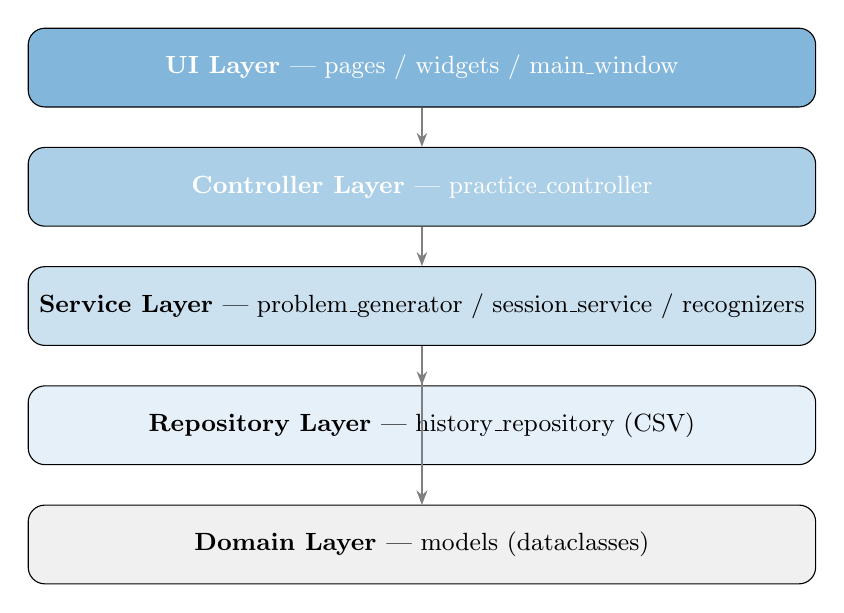
\begin{tikzpicture}[
    layer/.style={draw,rounded corners=6pt,minimum width=10cm,
                  minimum height=1cm,align=center,font=\small\bfseries},
    arr/.style={-{Stealth[length=5pt]},thick,gray},
    node distance=0.5cm
  ]
    \node[layer,fill=accent!60,text=white]   (ui)   {UI Layer \normalfont — pages / widgets / main\_window};
    \node[layer,fill=accent!40,text=white,below=of ui]  (ctrl) {Controller Layer \normalfont — practice\_controller};
    \node[layer,fill=accent!25,below=of ctrl] (svc)  {Service Layer \normalfont — problem\_generator / session\_service / recognizers};
    \node[layer,fill=accent!12,below=of svc]  (repo) {Repository Layer \normalfont — history\_repository (CSV)};
    \node[layer,fill=gray!12,below=of repo]   (dom)  {Domain Layer \normalfont — models (dataclasses)};

    \draw[arr] (ui)   -- (ctrl);
    \draw[arr] (ctrl) -- (svc);
    \draw[arr] (svc)  -- (repo);
    \draw[arr] (repo) -- (dom);
    \draw[arr] (svc)  -- (dom);
  \end{tikzpicture}
\end{frame}

% ------- Directory Structure -------
\begin{frame}[fragile]{Project Directory Structure}
\begin{lstlisting}[language={},basicstyle=\ttfamily\scriptsize]
arithmetic_helper/
  main.py                        # Entry point + .env loading
  app/
    domain/models.py             # PracticeConfig, PracticeQuestion,
                                 # AnswerRecord, SessionResult
    services/
      recognizer_backend.py      # RecognizerBackend (ABC)
      handwriting_recognizer.py  # sklearn SVM
      google_vision_recognizer.py
      baidu_ocr_recognizer.py
      tencent_ocr_recognizer.py
      tesseract_recognizer.py
      paddle_ocr_recognizer.py
      problem_generator.py       # Question generation engine
      session_service.py         # Session lifecycle management
    repositories/
      history_repository.py      # CSV persistence
    controllers/
      practice_controller.py     # Signal-driven UI orchestration
    ui/
      main_window.py             # Main window + dependency injection
      pages/  widgets/           # Pages & components
    i18n/localizer.py            # Internationalization
\end{lstlisting}
\end{frame}

% ------- Design Patterns -------
\begin{frame}{Key Design Patterns}
  \begin{columns}[T]
    \column{0.48\textwidth}
    \begin{block}{\faProjectDiagram\; Strategy Pattern}
      \texttt{RecognizerBackend} abstract base class\\
      6 concrete implementations, plug-and-play\\
      Runtime switching based on user selection
    \end{block}

    \vspace{6pt}
    \begin{block}{\faIndustry\; Factory Pattern}
      \texttt{MainWindow.\_build\_recognizer()}\\
      Instantiates backend by key string\\
      Built-in cache prevents duplicate creation
    \end{block}

    \column{0.48\textwidth}
    \begin{block}{\faSyringe\; Dependency Injection}
      \texttt{MainWindow} creates and wires all deps\\
      Service $\to$ Controller $\to$ Page\\
      Easy to mock for unit testing
    \end{block}

    \vspace{6pt}
    \begin{block}{\faBroadcastTower\; Signal / Slot Communication}
      PyQt signals drive UI updates\\
      Controller emits signals\\
      Pages subscribe and respond
    \end{block}
  \end{columns}
\end{frame}

% ------- Recognizer Abstract Class -------
\begin{frame}[fragile]{Recognizer Backend: Abstraction \& Extension}
\begin{lstlisting}[language=Python]
class RecognizerBackend(ABC):
    @abstractmethod
    def recognize(self, image: QImage) -> int | None:
        """Recognize handwriting, return integer or None"""

    @property
    @abstractmethod
    def name(self) -> str:
        """Human-readable backend name"""

    @property
    @abstractmethod
    def available(self) -> bool:
        """Whether dependencies / API keys are ready"""

    @staticmethod
    def _qimage_to_png_bytes(image: QImage) -> bytes | None:
        """Shared utility: QImage -> PNG bytes"""
\end{lstlisting}

  \vspace{4pt}
  \centering
  \tikz{\node[draw=good,rounded corners,fill=good!8,inner sep=6pt,text width=11cm,align=center]
    {Adding a new backend only requires inheriting this class and implementing 3 abstract members};}
\end{frame}

% ------- API Key Management -------
\begin{frame}[fragile]{Universal API-Key Interface}
  \begin{columns}[T]
    \column{0.5\textwidth}
    \begin{block}{Mechanism}
      \begin{enumerate}
        \item \texttt{main.py} loads \texttt{.env} at startup
        \item Writes to \texttt{os.environ}
        \item Each Recognizer reads required variables
        \item \texttt{available} property validates keys
      \end{enumerate}
    \end{block}

    \column{0.48\textwidth}
\begin{lstlisting}[language={}]
# .env example
GOOGLE_VISION_API_KEY=xxx
BAIDU_API_KEY=xxx
BAIDU_SECRET_KEY=xxx
TENCENT_SECRET_ID=xxx
TENCENT_SECRET_KEY=xxx
\end{lstlisting}
  \end{columns}

  \vspace{8pt}
  \centering
  \tikz{\node[draw=accent,rounded corners,fill=accent!8,
    inner sep=6pt,text width=12cm,align=center]{
    Users only need to edit the \texttt{.env} file to switch OCR providers — \textbf{zero code changes}
  };}
\end{frame}

% ------- Tech Stack -------
\begin{frame}{Technology Stack}
  \centering
  \renewcommand{\arraystretch}{1.4}
  \begin{tabular}{ll}
    \toprule
    \textbf{Layer} & \textbf{Technology} \\
    \midrule
    GUI Framework    & PyQt5 + qt-material theme \\
    Language         & Python 3.10+ \\
    Local OCR        & scikit-learn (SVM), Tesseract, PaddleOCR \\
    Cloud OCR        & Google Vision, Baidu OCR, Tencent Cloud OCR \\
    Persistence      & CSV (lightweight, portable) \\
    i18n             & Custom Localizer (zh\_CN / en\_US) \\
    Styling          & Material Design + custom CSS \\
    \bottomrule
  \end{tabular}
\end{frame}

% ------- Extensibility -------
\begin{frame}{Extensibility}
  \begin{columns}[T]
    \column{0.48\textwidth}
    \begin{block}{Current Capabilities}
      \begin{itemize}
        \item Four basic operations + mixed expressions
        \item 6 recognition backends
        \item Chinese / English interface
        \item CSV history storage
      \end{itemize}
    \end{block}

    \column{0.48\textwidth}
    \begin{block}{Future Directions}
      \begin{itemize}
        \item New problem types (fractions, equations \dots)
        \item New recognition backends (inherit ABC)
        \item New languages (extend dictionary)
        \item New storage (SQLite / cloud)
        \item Adaptive difficulty algorithms
      \end{itemize}
    \end{block}
  \end{columns}

  \vspace{10pt}
  \centering
  
\begin{tikzpicture}
    \node[draw=accent,rounded corners=10pt,fill=accent!8,
          inner sep=10pt,text width=11cm,align=center,font=\large]
      {Layered decoupling + abstract interfaces = \textbf{low-cost extensibility}};
  \end{tikzpicture}
\end{frame}

% ============================================================
\section{Summary}
% ============================================================

\begin{frame}{Summary}
  \begin{enumerate}
    \setlength{\itemsep}{10pt}
    \item \textbf{Product}: Clean UI + handwriting recognition + rich history $\to$ child-friendly practice experience
    \item \textbf{Cost Advantage}: Deterministic code generation, zero marginal cost, 100\% correct
    \item \textbf{Engineering Quality}: Five-layer decoupled architecture with Strategy / Factory / DI patterns
    \item \textbf{Flexible Extension}: Abstract recognizer interface + universal API-Key management $\to$ plug-and-play
  \end{enumerate}

  \vspace{16pt}
  \centering
  {\Large\bfseries\textcolor{accent}{Thank You!}}\\[6pt]
  {\small Questions \& Discussion}
\end{frame}

\end{document}
